\section{Architecture and Implementation}
\label{sec:architecture}

%%%%%%%%%%%%%%%%%%%%%%%%%%%%%%%%%%%%%%%%%%%%%%%%%%%%%%%%%%%%%%%%%%%%%%%%%%%%%%%%%%%%%%%
% Intro to arch
%%%%%%%%%%%%%%%%%%%%%%%%%%%%%%%%%%%%%%%%%%%%%%%%%%%%%%%%%%%%%%%%%%%%%%%%%%%%%%%%%%%%%%%

To address the concerns outlined in the previous section we introduce two
new abstractions: safe collections, an abstraction that encapsulates
a dataset and the set of policies that govern its use; and stewards, privileged users
to manage safe collections while separating administrative from infrastructure
administrators.  
In this model, administrators first define a safe collection and declare one 
or more stewards to manage that collection. This process transfers
all administrative responsibilities regarding access and export of data to the stewards.
%who now take ownership and responsibility for the safe collection.

\subsection{Safe Collection}

Datasets come with various levels of sensitivity. Selecting the policies, protocols, infrastructure, and 
software settings to ensure to ensure that individual datasets are adequately secured requires
case-by-case consideration. To represent these policies, such that dataset owners can manage these considerations
we define safe-collections. Safe-collections enable system administrators to partition the key administration
aspects of managing the relationship between analysts (data users/accessors) and data. 
Safe-collections encapsulate a data-store where the dataset will reside, and a consistent set of policies
that controls access to the data-store as well the policies themselves.

We extend our AWS-based Cloud Kotta services by leveraging additional
services and guarantees provided by AWS. 
Safe-collection policies are expressed on CLoud Kotta's S3-hosted data
%The data-store is implemented over S3 object store, and the
using Identity and Access Management(IAM) policies and S3 bucket policies.
A safe-collection is described in cloudformation, a JSON-based software defined infrastructure model for AWS.
This allows safe-collection descriptions to be verifiable, reproducible, and shareable.

Safe-collections offer a range of policies including specification of limits as well as management 
of access, usage, and data export. We define a meta-policy model via which administrators may define
the set of policies permissible on a safe-collection. Each safe-collection is associated with a steward
(or group of stewards) who may manage safe-collection policies. To simplify use, the meta policy schema 
is translated to a web-based form that can be completed by users during creation of a safe-collection. 
The completed form is stored as a set of special tags on the collection's data storage. The schema is enforced
by the various services that interact with the safe-collection. The schema and the generated form are shown in
\figurename~\ref{fig:schema}

\begin{figure*}[ht]
  \center
  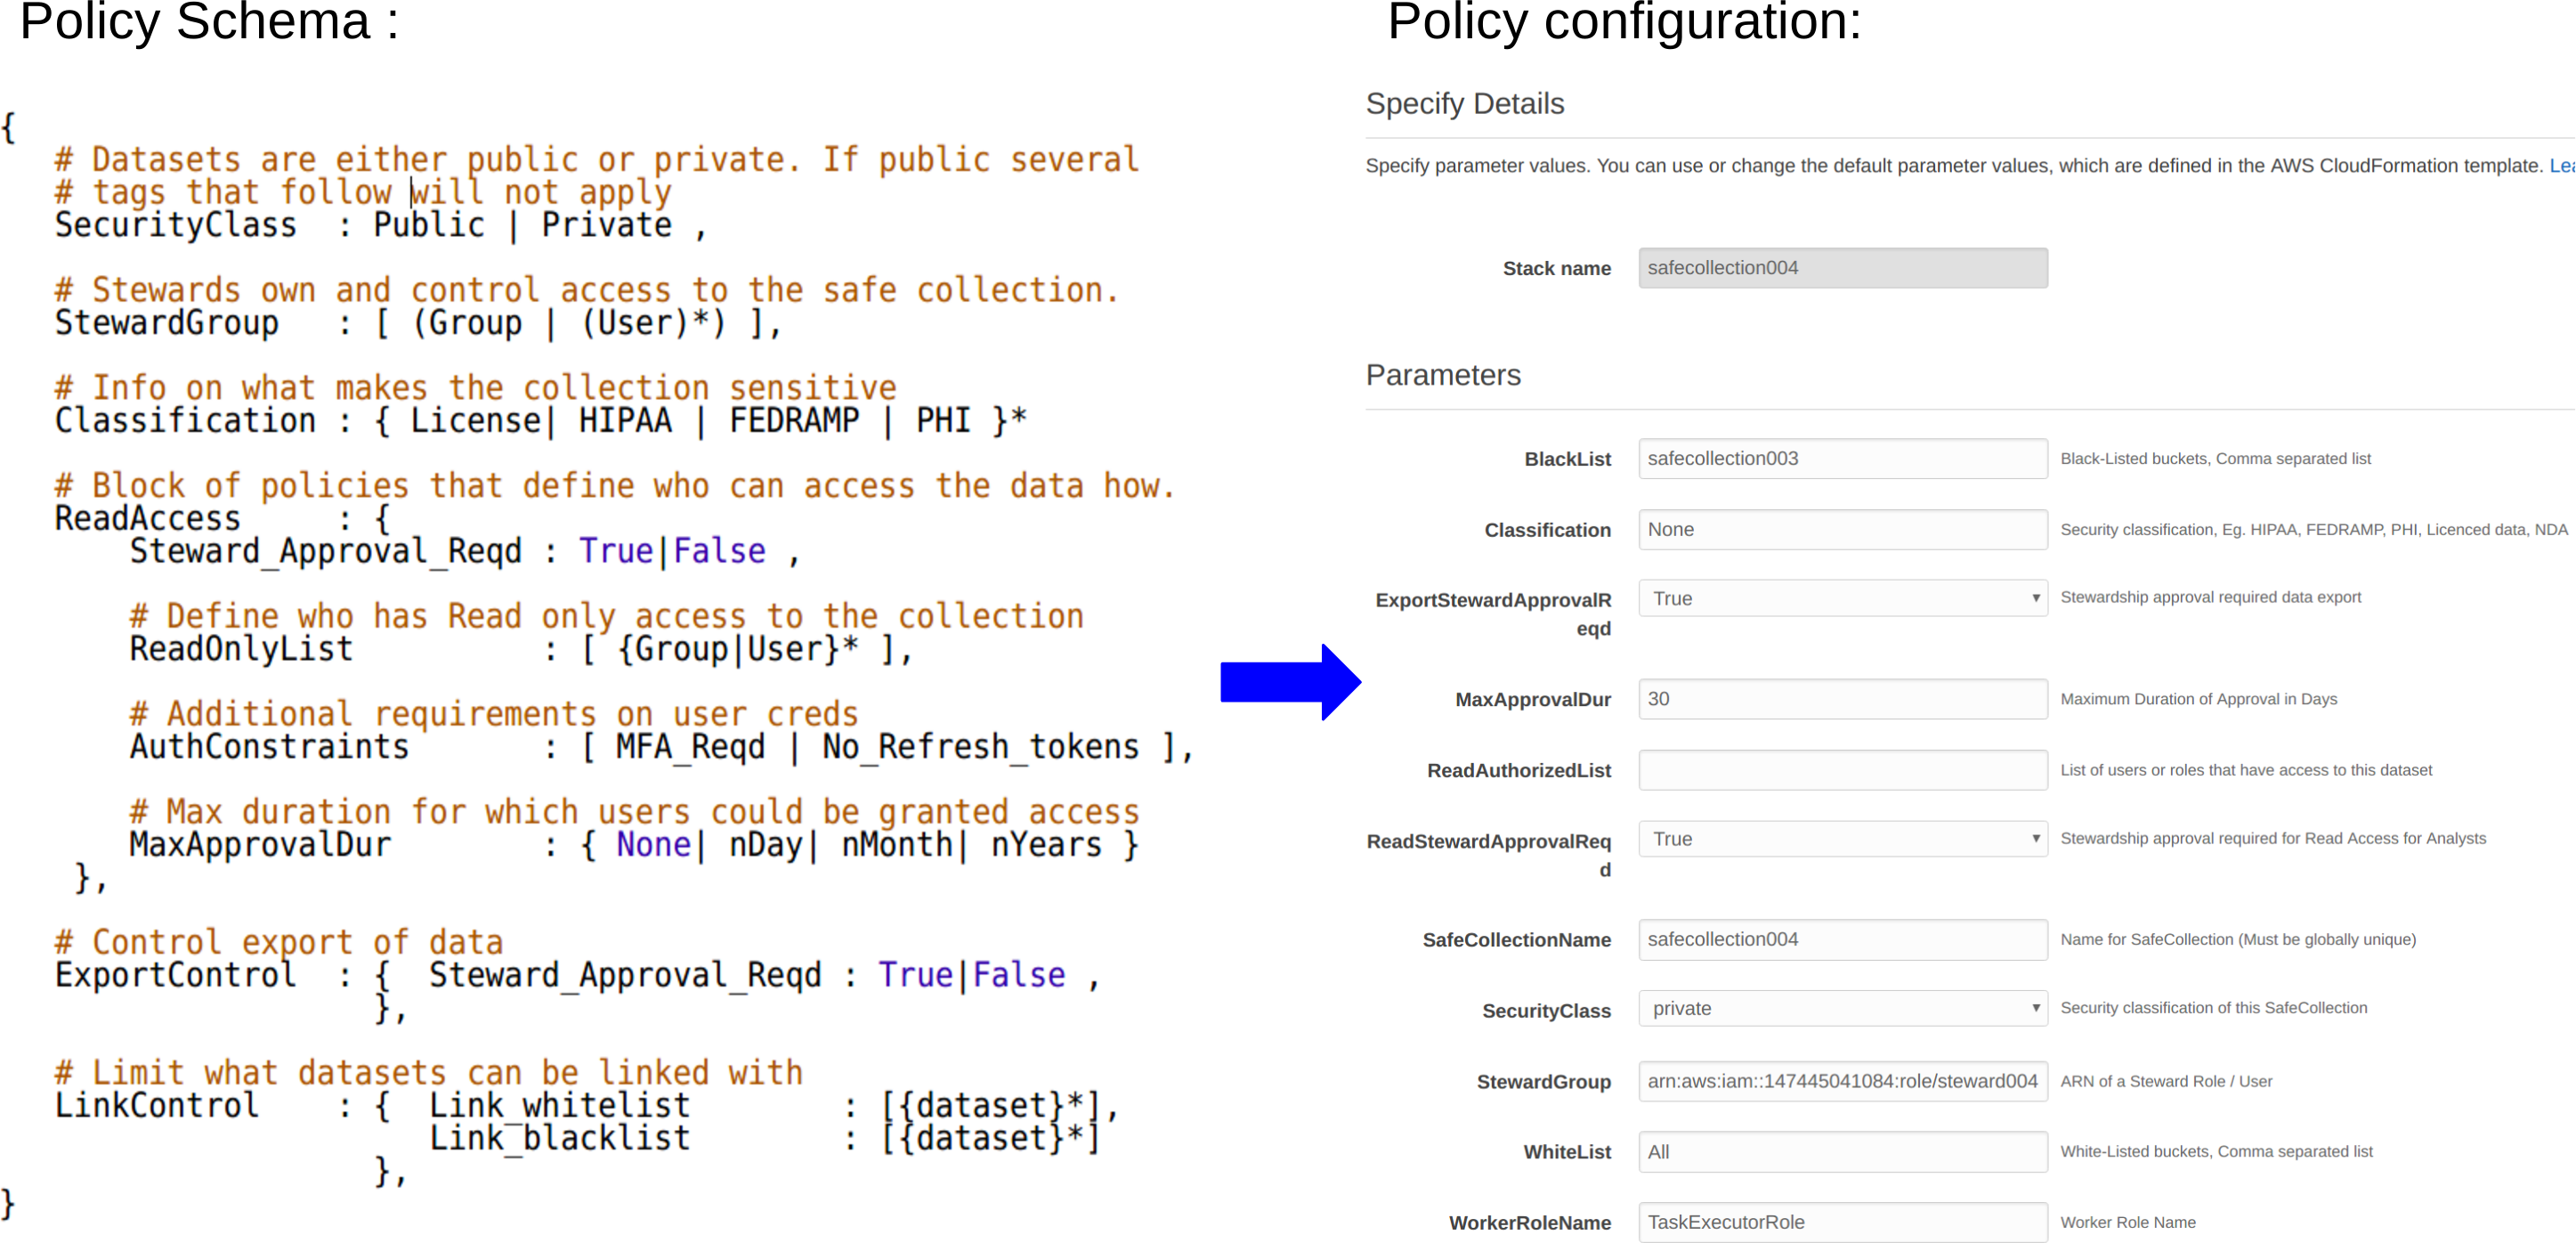
\includegraphics[width=\textwidth, height=8cm]{figures/meta-policy.png}
  \caption{Meta-policy specification and configuration}
  \vspace{-1.5em}
  \label{fig:schema}
\end{figure*}

% Public data
Public datasets are assumed to contain no sensitive content and thus do not require access control nor
export control. Setting \texttt{SecurityClass} to \texttt{Public} indicates that the safe-collection does
not require a Steward and that all authenticated users on \NAME may access this dataset. None of the added
security features of safe-collections need apply.

% Common features for private data
Confidential and regulated datasets both require \texttt{SecurityClass} to be set to \texttt{Private}
and require that a steward group is specified. In addition, constraints can be set on the duration
for which analysts could be granted access. This ensures that access privileges expire and require
re-evaluation of the scope and nature of the analyst's work before access is extended. To limit the risk of
re-identification in datasets that contain anonymized data the safe-collections allow for whitelisting and
blacklisting other safe-collections. Job submissions to \NAME are checked for data requests that have
linkage conflicts, and denied at submit time.
\yadu{Linkage feature pending}

% implementation of access control
Access control on safe-collections for private datasets are managed by stewards. Access privileges to
safe-collections are granted, extended and revoked via S3 bucket policies. At the time of creation all
privileges over bucket policies are granted to the steward and revoked for all other entitites. This
guarantees that only the stewards can grant privileges on safe-collection. Access is granted by stewards
by adding a new bucket policy conditional on an expiration deadline. These policies may be revoked or
extended by updating the expiration deadline, thus offering fine-grained control to stewards on managing
access.

% cite garfinkel for de-identification risks

Safe-collections that contain regulated datasets often require oversight to ensure that all computed results
are inspected and approved by a steward before export. This is enforced by setting the
\texttt{ExportStewardApprovalReqd} flag.
Analysis results from tasks that consumed data from any safe-collection with this flag has all of the
results posted back to the same safe-collection, thus inheriting the same privileges as the source.
% worker roles are granted write privileges to the outputs section of a safe-collection
As a result, only stewards can view the results and export to a public safe-collection. Since results are
stored within the parent safe-collection, users can apply analysis operations on results without oversight,
and only request for export of the final results of a deep analysis pipeline.

\subsection{Stewardship}

% Why do we have them / inital role
As more data-sets with varying degrees of sensitivity are added to the \NAME platform it becomes a matter
of necessity to distribute key administrative privileges from the system administrator roles to the curators
of the data-set. Stewards play a leadership role in evaluating the disclosure risks associated with a
dataset and codifying the security protocols protecting the safe-collection.

% implementation details
Upon creation of a safe-collection a single steward group implemented as an IAM role, is added to the
access policies of the safe-collection. This steward role is the sole entity on the platform capable of
updating polices attached to the safe-collection.
Multiple users could be associated with a steward role and is recommended, so that requests can be served quicker.
Once user identities are established by authenticating with an external identity provider,
\NAME allows users to ``assume'' a privileged IAM role that they have been attached to.
By assuming the steward role, a user temporarily gains the privileges to carry out operations such
as updating access policies and exporting data from a safe-collection.
Once created the steward's responsibilities are two-fold: arbitrate access requests to the safe-collection and
handle export requests for results generated from safe-collections.

% access
Analysts can list all available safe-collections and request access to ones that they require.
Stewards evaluate these requests and approve access for a duration. Approvals are implemented as an additional
policy added to the list of s3 bucket policies for the safe-collection. \NAME ensures that the policy
being added is consistent with the meta-policy for the safe-collection, for eg. expiration for the policy
must be within the duration specified in the \texttt{MaxApprovalDur}.
\yadu{pending}

% export
On export controlled safe-collections, results generated by analysis tasks on \NAME are not visible to the
analysts until approved by a Steward. This is implemented by having workers write all results to the
parent safe-collections output directory and thus inheriting the same security privileges of the parent.
On \NAME stewards have complete visibility over the set of inputs, and operations made by the analysts
in order to generate their results. It is also possible to trace the provenance of the results from an
analysis pipeline since all analysis tasks are logged.
Stewards export the results by transferring the results out of the safe-collection and onto a public
safe-collection from which analysts can view results. It is important to note that even public
safe-collections have server side encryption and are only accessible to authenticated users via temporary
signed urls.


\subsection{User Flows}

Here we describe the two most common flows introduced by this model:

\subsubsection{Access Flow}

Bob an analyst authenticates on the system and requests access to a private safe-collection.
The request is now visible on the stewarship dashboard of all stewards. Alice, a steward for the requested
safe-collection approves the request for n days. The approval process adds the appropriate policies to the
safe-collection granting access to Bob. Bob now can submit tasks via the  REST api, that specify data-items
from the safe-collection as inputs. The REST api marks the task as export controlled since it draws results
from an export controlled safe-collection. The submitted task is posted to an internal queue from which a
worker node in the \NAME private subnet picks up Bob's task. The worker node assumes Bob's identity and with
his credentials requests data from the safe-collection. Since Bob now has read privileges for the
safe-collection, the data is fetched to the worker node, on which the analysis task is executed.
Upon completion, the worker node puts the generated results under the outputs directory of the safe-collection
since the task used export controlled data. Bob's analysis is now complete, but he is unable to view the
results. This flow is show in \figurename~\ref{fig:flow1}

\begin{figure}
  \center
  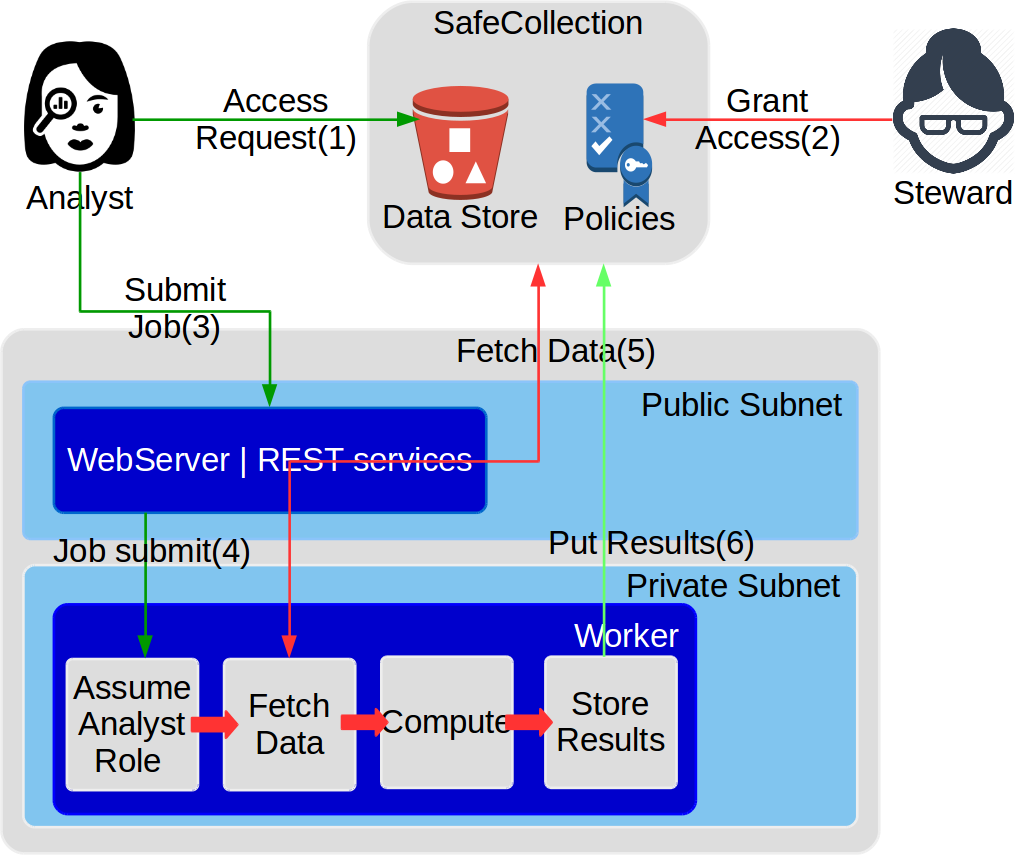
\includegraphics[width=0.45\textwidth]{figures/safe_flow.png}
  \caption{Safe collection schema}
  \label{fig:flow1}
  \vspace{-1.5em}
\end{figure}


\subsubsection{Export Flow}

Once Bob's analysis task is complete Bob realizes that he requires export approval before he may view the
results, so he issues a request for export. Alice, sees a new export request on her dashboard. Alice assumes
the steward role with a fresh authenticated token, and accesses the results and the complete description
of Bob's analysis task. Once Alice deems the results safe for export, she initiates data export. \NAME
services use Alice's temporary credentials to transfer the results from the safe-collection to a public
safe-collection and updates the task information with new location of the results. Bob can now log on
and view or download the results. This flow is show in \figurename~\ref{fig:flow2}

\begin{figure}
  \center
  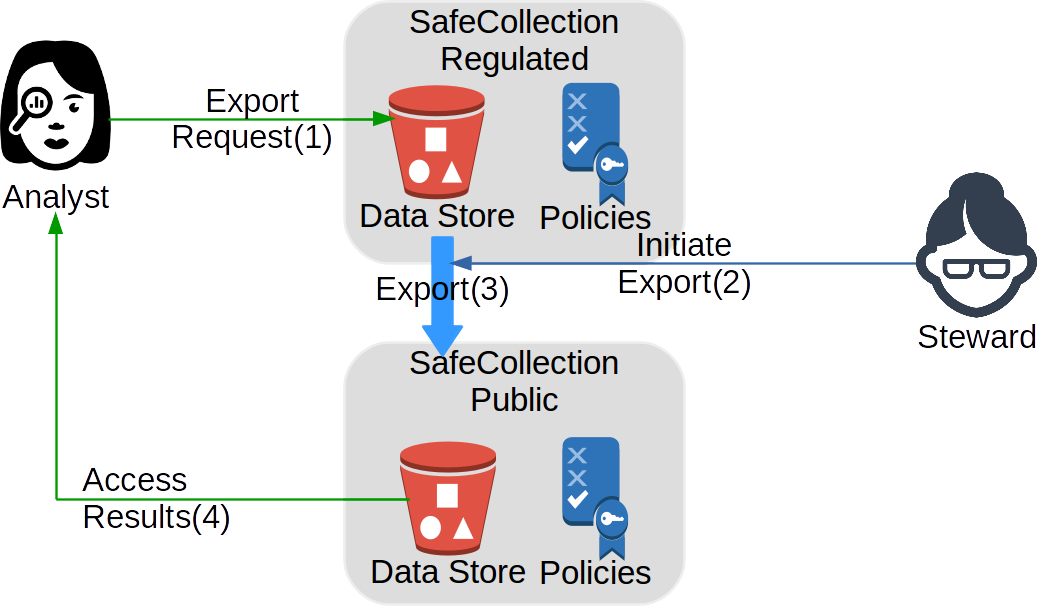
\includegraphics[width=0.45\textwidth]{figures/export_flow.png}
  \caption{Safe collection schema}
  \label{fig:flow2}
  \vspace{-1.5em}
\end{figure}









